%\documentclass{beamer}
\documentclass[handout]{beamer}
\setbeamercovered{transparent}

\usepackage[utf8]{inputenc}

\usepackage[german]{babel}
\usepackage{color}
\usepackage{xcolor}
\usepackage{graphicx}
\usepackage{tikz}
\usepackage{design_latex-template/beamerthemeFOSSAG}
\usepackage{subfiles}
\usepackage{hyperref}

 


\title{SSH}
\subtitle{Kontrolle aus der Ferne}
\author{@innaytool [Yannick Bungers] \\ innay@foss-ag.de}
\institute{\textcolor{blue}{\href{https://foss-ag.de} {\underline{FOSS AG}}}\\ \href{https://github.com/foss-ag/vortrag\_ssh}{git@github.com:foss-ag/vortrag\_ssh.git}}
\date{\today}

\begin{document}

\begin{frame}
\titlepage
\end{frame}

% Dateien
%\subfile{content.tex}
\subfile{motivation.tex}
\subfile{history.tex}
\subfile{introduction.tex}
%\subfile{test.tex}
\subfile{software.tex}
%\subfile{sshsub.tex}
\subfile{sftp.tex}
\subfile{scp.tex}
\subfile{sshfs.tex}
\subfile{remoteexec.tex}
%\subfile{porttunnel.tex}
\subfile{socks5.tex}
\subfile{localtunnel.tex}


\begin{frame}
	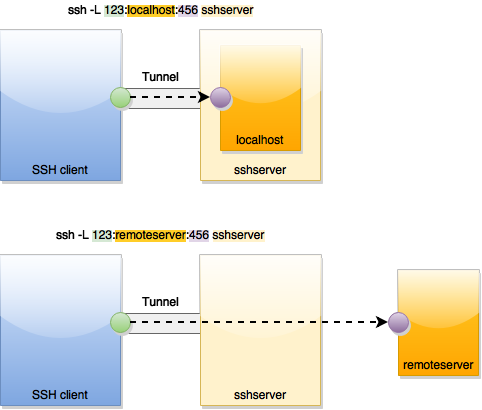
\includegraphics[scale=0.55]{ssh-L-tunnel.png}
\end{frame}

\subfile{remotetunnel.tex}

\begin{frame}
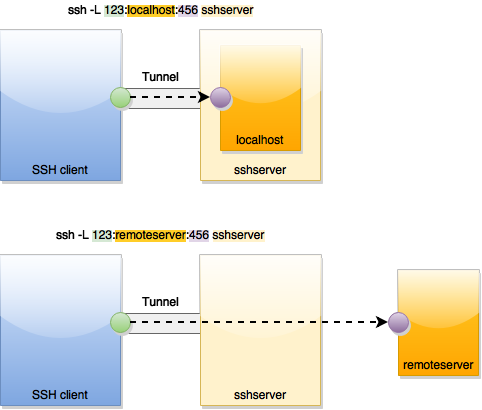
\includegraphics[scale=0.55]{ssh-L-tunnel.png}
\end{frame}

\subfile{server.tex}
\subfile{sshkey.tex}
\subfile{summary.tex}
\end{document}
